
\section{Experiments}
\label{sec:experiments}

In this section, we wish to experimentally evaluate two criteria: the
performance of the different optimisation algorithms to minimise the \addkrrs
objective \eqref{eqn:optObjective}, and the performance of \addkrrs and other
nonparametric regression methods. So far, we only have results on synthetic
data.

\subsubsection*{Experimental set up}
For our synthetic experiments, we take $\Xcal = [-1, 1]^D$.
We constructed a function of $3$ modes by taking the logarithm of $3$
Gaussian bumps whose centres are randomly chosen from $\Xcal$.
We uniformly randomly sample $500$ points each for training and testing from
$\Xcal$ and uses the true function values as the labels.
In the examples we consider below we take $D = 20$, $d = 4$ and $M = 50$. 
Therefore, our optimisation problem had $50 \times 500 = 25,000$ parameters.


\subsubsection*{Comparison of Optimisation Algorithms}
We compared the five methods specified above on the synthetic example outlined
above. Figures~\ref{fig:iteration} and~\subref{fig:time} shows the improvement
in the objective over iterations and time respectively over $2000$ iterations. 
\subgrad and \proxgrad exhibit slow convergence but
\proxgradaccn, \bcdexact and \bcgddiag perform quite well. 
\proxgradaccn does marginally better than the rest.
Even for different values of $D$, $d$, $M$  we found that the latter three
methods did better but their relative performances varied slightly.
In our experiments below we use \proxgradaccn.

\subsubsection*{Comparison with other Regression Algorithms}
We use the same experimental set up as explained above to compare \addkrrs
against the \krrs and \nws methods. To choose the kernel bandwidth for \nws  
we used $5$-fold cross validation. Due to time constraints, parameter selection 
 for \addkrrs and \krrs was very coarse -- we tried only $5$ different choices
for $(\lambda_1, \lambda_2)$ and used $2$-fold cross validation.
Despite this, \addkrrs significantly ourperforms both \krrs and \nws on the
synthetic problem. The results are depicted in Figure~\ref{fig:compare}. These
results are quite encouraging as they attest well to our intuitions about
favourable bias variance tradeoffs when using (statistically simpler) additive
models for high dimensional regression.

\begin{figure*}
\centering
\subfigure[]{
  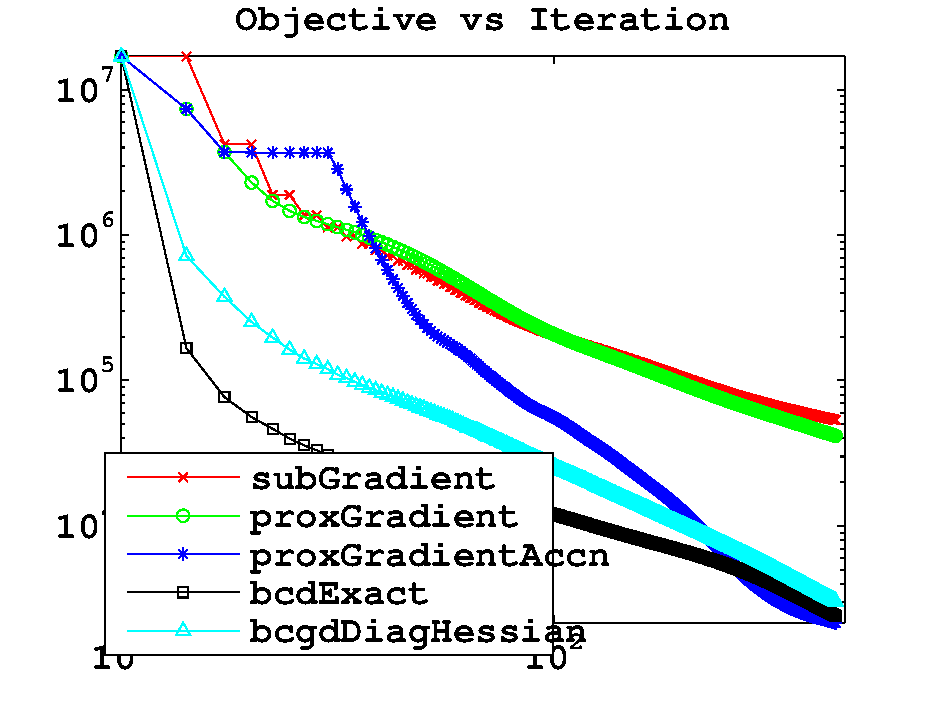
\includegraphics[width=\imarrwthree]{figs/iteration2000v1} \hspace{\imhspthree}
  \vspace{\imlabelspace}
  \label{fig:iteration}
}
\subfigure[]{
  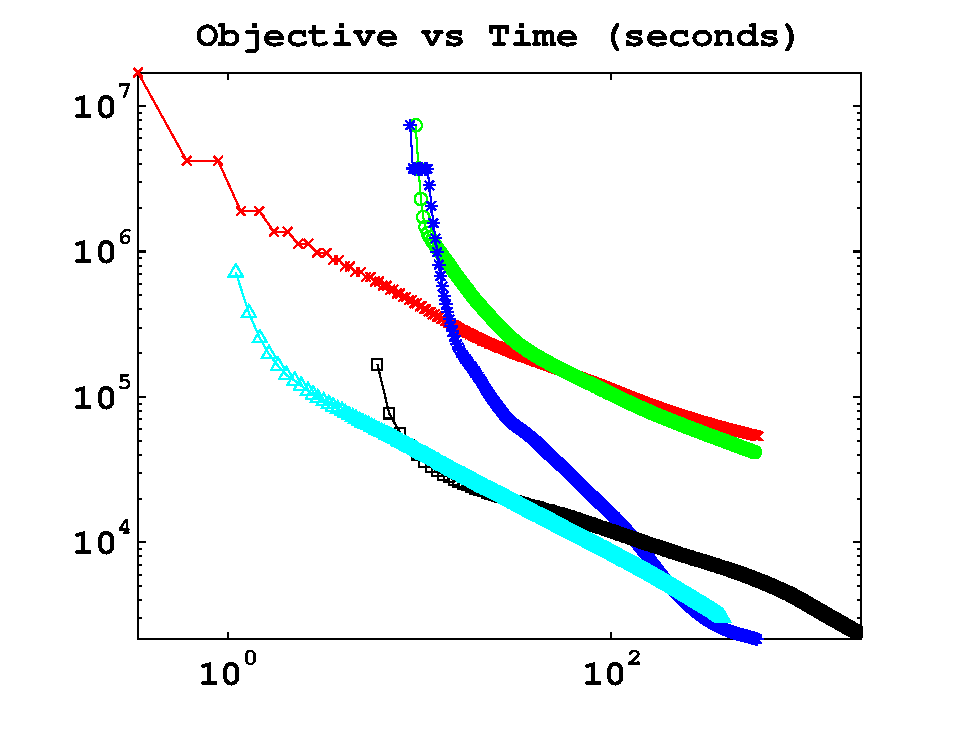
\includegraphics[width=\imarrwthree]{figs/time2000v1} \hspace{\imhspthree}
  \vspace{\imlabelspace}
  \label{fig:time}
}
\subfigure[]{
  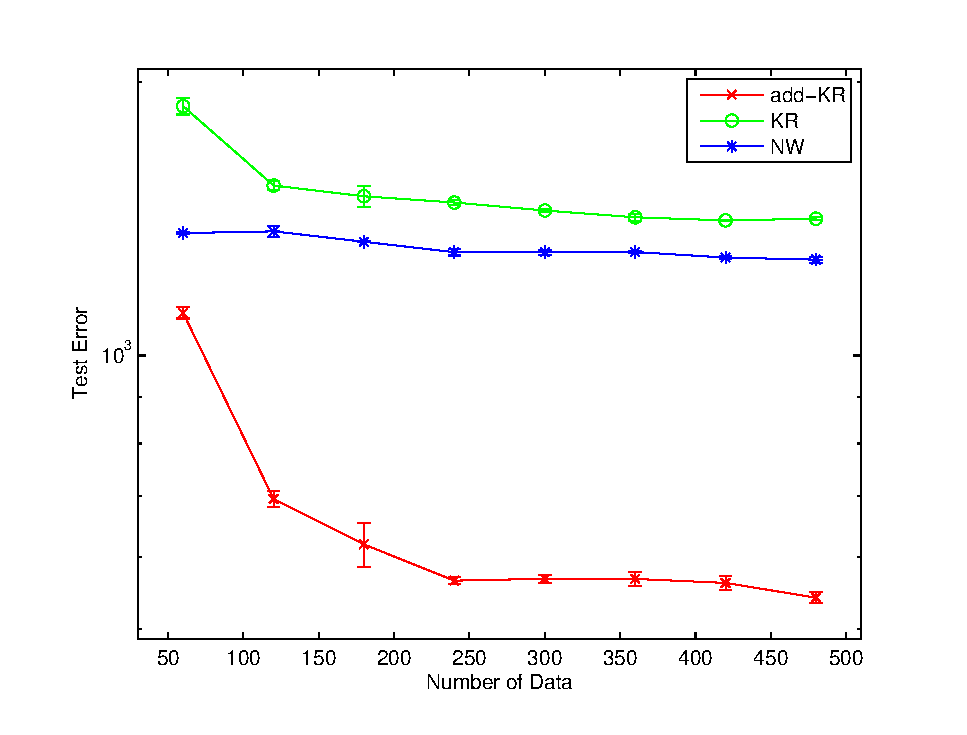
\includegraphics[width=\imarrwthree]{figs/toyResults}
  \vspace{\imlabelspace}
  \label{fig:compare}
} \\
\caption[]{ \hspace{-0.1in}
Figures~\subref{fig:iteration} and~\subref{fig:time} plot the objective value vs
iteration and cpu time respectively. Accelerated proximal gradient descent (blue
curve) seems to perform best. Figure~\subref{fig:compare} plots the test set
error for \addkrrs, \krrs and \nws on a synthetic problem. 
\addkrrs outperforms both methods.
We apologise for the small labels as we were running short of time.
}
\label{fig:toythree}
\vspace{\imtextspace}
\end{figure*}

